\subsection{Upgrade Design of the Protocol Code}

We first give the block structure of the Nebulas, and then discuss how to upgrade the protocol code based on the block structure.

\subsubsection{Block Structure}

The Nebulas block data structure contains, but is not limited to, the following:

\begin{itemize}
	\item Header: Block Header
		\begin{itemize}
		\item Height:block height
		\item ParentHash:parent block hash
		\item Ts:timestamp
		\item Miner:miner address
		\item Dynasty:the consensus dynasty of the block
		\item Epoch:the consensus age of the block
		\item StateRoot:state root hash
		\item TxsRoot:transaction root hash
		\item ReceiptsRoot:transaction receipt hash
		\item TransNum:number of transactions
		\end{itemize}
	\item Transactions:transaction data (including multiple transactions)
		\begin{itemize}
		\item From:transaction sender address
		\item To:transaction receiver address, for creating a smart contract with a value 0x0
		\item Value:transfer amount
		\item Data:Transaction payload. It's the smart contract bytecode if the transaction is for creating a smart contract; It's the name of the calling function and the entry if the transaction is a smart contract call.
		\item Signature:transaction signature
		\item Gas:gas limit
		\item GasPrice:gas unit price
		\item Nonce:the uniqueness of transactions
		\end{itemize}
	\item Votes:Prepare and Commit Votes (including multiple), used in PoD (see \refsec{sec:pod}) consensus algorithm
		\begin{itemize}
		\item From:voter
		\item VoteHash:hash of the block voted for
		\item Hv:the height of the block voted for
		\item Hvs:the height of an ancestral block of the block voted for
		\item VoteType:voting type,Prepare or Commit
		\item Signature:vote signature
		\end{itemize}
	\item Protocol Code:The protocol code (only 0 or 1 in a block)
		\begin{itemize}
		\item Hash:hash of the protocol code
		\item Code:the bytecode of the protocol code
		\item ValidStartBlock:the start block number that protocol come into effect
		\item Signature:signautre (sign by the developer community)
		\item Version:the protocol code version number, and each upgrade needs to be incremented to prevent malicious accounts from rolling back to the old protocol code
		\item Nonce:the uniqueness of protocol code
		\end{itemize}
	\item Nebulas Rank:Nebula index (calculated once a week, most blocks haven't this section)
		\begin{itemize}
		\item RankVersion:NR version
		\item RankRoot:NR rank hash
		\item RankRecords:NR rank record
			\begin{itemize}
				\item Address:Account address tag
				\item Score:NR value
			\end{itemize}
		\end{itemize}
\end{itemize}

\begin{figure}[!h]
\centering
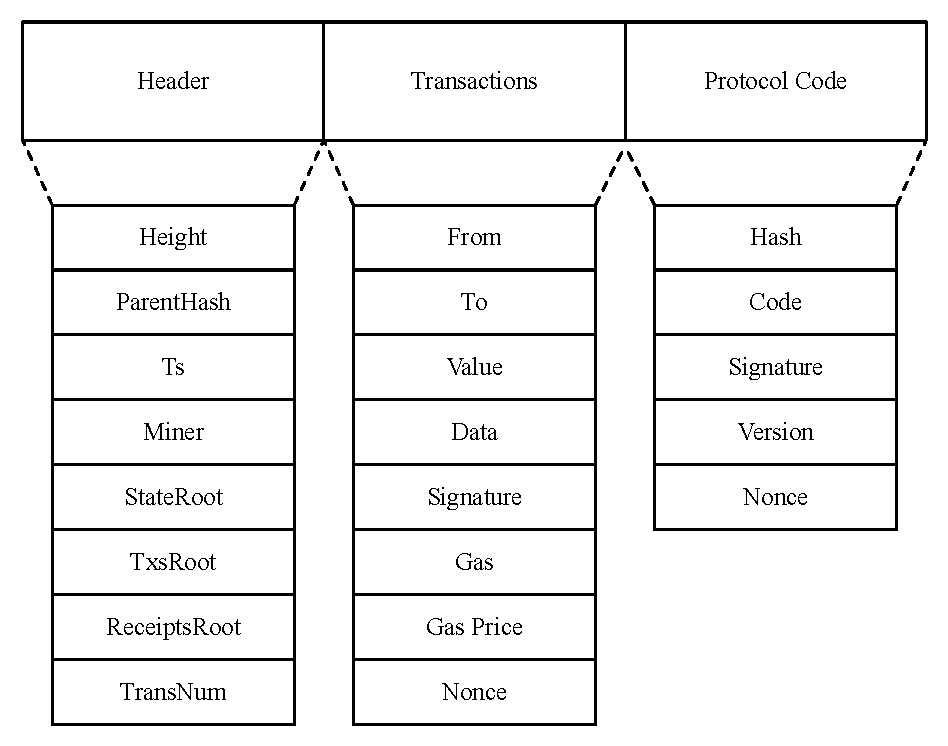
\includegraphics[width=13.8cm]{./figs/block}
\caption{Block Structure}
\label{fig:block}
\end{figure}

Similar to other cryptocurrency systems, the interaction between the account and the blockchain is done through a particular transaction. The account creates a transaction, which is signed with a private key, and sends it to any node in the blockchain and broadcasts it to full network node through the P2P network. During the fixed block time interval, the nodes specified by the PoD consensus algorithm (see \refsec{sec:pod}) collect all transactions in the time and pack them into blocks of standard format and broadcast them to the rest of the network. After verification by each node, the new block is appended into the local ledger and becomes a part of the global ledger.

In Ethereum, transactions are divided into two types: ordinary account transaction and smart contract transaction. We add new transaction types to the blocks of Nebulas: protocol code and the Nebulas Rank. The protocol code, as a part of the blockchain data, is stored on the chain, and the upgrade of the basic protocol of Nebulas is carried out through supplementing additional data on chains. Based on the NR ranking algorithm, the NR value of each account is calculated in each cycle and saved in the corresponding chain to facilitate the real-time NR value calling and historical ranking query.

\subsubsection{Upgrade of the Protocol Code}

The Nebulas client node can obtain the compiled virtual machine bytecode (NVM bytecode) from the storage area of the Protocol Code in the latest block. If there are no data of the Protocol Code in the latest block, it indicates that the protocol code has no change and has to trace back to the Protocol Code in the nearest block. Any actions of the protocol code of blockchains will be determined by the Protocol Code, including the authentication algorithm, the packing rules, the NR algorithm, the incentive mechanism, etc. Almost all actions of blockchains can be defined by the Protocol Code.

If the protocol code needs to be upgraded, the Nebulas development team will be responsible for its development and the code will be released to open channels for discussion and voting in communities. Voting can be carried out in the form of the smart contract or voting in the forum. If the majority of community members agree to upgrade the protocol, the Nebulas development team will pack the latest code into Protocol Code transaction, and release it to all nodes of the whole network; only if the bookkeeping nodes include it in blocks, it will become valid at the specified block height. This type of blockchain protocol upgrade is transparent to clients without soft and hard fork.

In order to ensure that the protocol code is released after authorization, the publisher of the Protocol Code uses the address reserved by the core Nebulas, cannot be changed with hard code within the genesis block. All bookkeeping nodes will verify the signature of Protocol Code. If the signature fails to pass the verification, it will be deemed as the illegal data.

The subsequent improvement measure is to change the signature verification of the Protocol Code into the M-of-N multi-signature, which can also be implemented through the upgrade of the Protocol Code.